 \documentclass{article}
\usepackage[utf8]{inputenc}
\usepackage[a4paper, total={7in, 10in}]{geometry}
\usepackage{braket}
\usepackage{xcolor}
\usepackage{amsmath}
\usepackage{amssymb}
\usepackage{amsfonts}
\usepackage{graphicx}
\usepackage{svg}
\usepackage{float}
\usepackage{tikz}
\usepackage[ruled,vlined]{algorithm2e}
\usepackage{multicol}
\usepackage[backend=biber,style=alphabetic,sorting=ynt]{biblatex}
\usepackage{xcolor}
%\addbibresource{sample.bib} %Import the bibliography file

\newcommand{\commentt}[1]{\textcolor{blue}{ \textbf{[COMMENT]} #1}}
\newcommand{\ctt}[1]{\commentt{#1}}
\newcommand{\prb}[1]{ \mathbf{Pr} \left[ {#1} \right]}
\newcommand{\onotation}[1]{\(\mathcal{O} \left( {#1}  \right) \)}
\newcommand{\ona}[1]{\onotation{#1}}
\newcommand{\PSI}{{\ket{\psi}}}
\newcommand{\LESn}{\ket{\psi_n}}
\newcommand{\LESa}{\ket{\phi_n}}
\newcommand{\LESs}{\frac{1}{\sqrt{n}}\sum_{i}{\ket{\left(0^{i}10^{n-i}\right)^{n}}}}
\newcommand{\Hn}{\mathcal{H}_{n}}
\newcommand{\Ep}{\frac{1}{\sqrt{2^n}}\sum^{2^n}_{x}{ \ket{xx}}}
\newcommand{\HON}{\ket{\psi_{\text{honest}}}}
\newcommand{\Lemma}{\paragraph{Lemma.}}


\setlength{\columnsep}{0.6cm}

\newcommand{\Gz}{ G_{z}^{\delta} } 

\begin{document}

\title{Quantum LTC With Positive Rate}
\author{David Ponarovsky}
\maketitle
\begin{multicols*}{2}
\newcommand{ \Hw }{ \delta\Delta -\Delta^{\frac{1}{2}-\varepsilon}/\delta  }
	\newcommand{ \Nw }{ \Delta^{\frac{3}{2}-\varepsilon}} 
	  \newcommand{ \Gu } { \Gamma^{\cup} }
	  \newcommand{ \Guq } { \Gamma^{\cup, \square} }

    	\newcommand{ \Gsa } {\Gamma_{\square_{1}} }
	\newcommand{ \Gsb } {\Gamma_{\square_{2}} }
        \newcommand{ \Aa } { C_{A_{1}}}  
	\newcommand{ \Ab } { C_{A_{2}}}
	\newcommand{ \Ac } { C_{A_{3}}}
	\newcommand{ \Aab } { \Aa \otimes \Ab } 
	\newcommand{ \Aac } { \Aa \otimes \Ac }
	\newcommand{ \Aabc } { \Aa \otimes \Ab \otimes \Ac }
	\newcommand{ \Aabp } { \Aa^{\perp} \otimes \Ab^{\perp} } 
	\newcommand{ \Aacp } { \Aa^{\perp} \otimes \Ac^{\perp} }
	\newcommand{ \Aabcp } { \Aa^{\perp} \otimes \Ab^{\perp} \otimes \Ac^{\perp} }
	\newcommand{ \Aabpp } { \left( \Aabp \right)^\perp } 
	\newcommand{ \Aacpp } { \left( \Aacp \right)^\perp }
	\newcommand{ \Aabcpp } { \left( \Aabcp \right)^\perp }
	\newcommand{ \YY } {  y_{1}y_{2}^{\top} }
	\newcommand{ \ZZ } {  z_{1}z_{2}^{\top} } 
	\newcommand{ \TT } { \tilde{\tau} } 


  \paragraph{preamble.} preamble.  
  \begin{figure}[H]
            %\label{fig:square}
            \begin{center}
            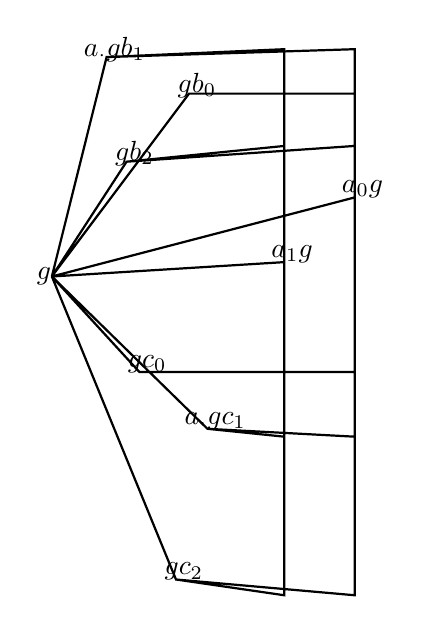
\begin{tikzpicture}
            \draw[thick](0,0)(0,0) -- (1.7426256721294677,2.3223750886338372) -- (3.8452742257941703,2.3223750886338372) -- (3.8452742257941703,1.0038904441049445) -- (0,0)
(0,0) -- (0.6952554722651207,2.786573979742071) -- (3.8452742257941703,2.8865739797420713) -- (3.8452742257941703,1.0038904441049445) -- (0,0)
(0,0) -- (0.9488861302609535,1.4578598738546527) -- (3.8452742257941703,1.6578598738546526) -- (3.8452742257941703,1.0038904441049445) -- (0,0)
(0,0) -- (1.7426256721294677,2.3223750886338372) -- (2.9507365622757,2.3223750886338372) -- (2.9507365622757,0.18240215250869518) -- (0,0)
(0,0) -- (0.6952554722651207,2.786573979742071) -- (2.9507365622757,2.8865739797420713) -- (2.9507365622757,0.18240215250869518) -- (0,0)
(0,0) -- (0.9488861302609535,1.4578598738546527) -- (2.9507365622757,1.6578598738546526) -- (2.9507365622757,0.18240215250869518) -- (0,0)
(0,0) -- (1.111570283305451,-1.2128803025270027) -- (3.8452742257941703,-1.2128803025270027) -- (3.8452742257941703,1.0038904441049445) -- (0,0)
(0,0) -- (1.9757529088749173,-1.9344114058313568) -- (3.8452742257941703,-2.034411405831357) -- (3.8452742257941703,1.0038904441049445) -- (0,0)
(0,0) -- (1.5764002244563355,-3.8482341519334247) -- (3.8452742257941703,-4.048234151933425) -- (3.8452742257941703,1.0038904441049445) -- (0,0)
(0,0) -- (1.111570283305451,-1.2128803025270027) -- (2.9507365622757,-1.2128803025270027) -- (2.9507365622757,0.18240215250869518) -- (0,0)
(0,0) -- (1.9757529088749173,-1.9344114058313568) -- (2.9507365622757,-2.034411405831357) -- (2.9507365622757,0.18240215250869518) -- (0,0)
(0,0) -- (1.5764002244563355,-3.8482341519334247) -- (2.9507365622757,-4.048234151933425) -- (2.9507365622757,0.18240215250869518) -- (0,0)
;
\node at (-0.1,0) {$ g $};
\node at (3.9452742257941704,1.1038904441049446) {$ a_{ 0 }g $};
\node at (3.0507365622757,0.28240215250869516) {$ a_{ 1 }g $};
\node at (1.8426256721294678,2.4223750886338373) {$ gb_{ 0 } $};
\node at (0.7952554722651207,2.8865739797420713) {$ a_{\cdot} gb_{ 1 } $};
\node at (1.0488861302609536,1.5578598738546527) {$ gb_{ 2 } $};
\node at (1.2115702833054511,-1.1128803025270027) {$ gc_{ 0 } $};
\node at (2.075752908874917,-1.8344114058313568) {$ a_{\cdot} gc_{ 1 } $};
\node at (1.6764002244563356,-3.7482341519334246) {$ gc_{ 2 } $};

            \end{tikzpicture}
            \end{center}
            \caption{Square of the complex, with edges $(g,ag), (agb, gb) \in E_A,
            (g,gb), (agb, ag) \in E_B.$ \label{fig:square}
            }
            \end{figure}
 \begin{figure}[H]
            %\label{fig:square}
            \begin{center}
            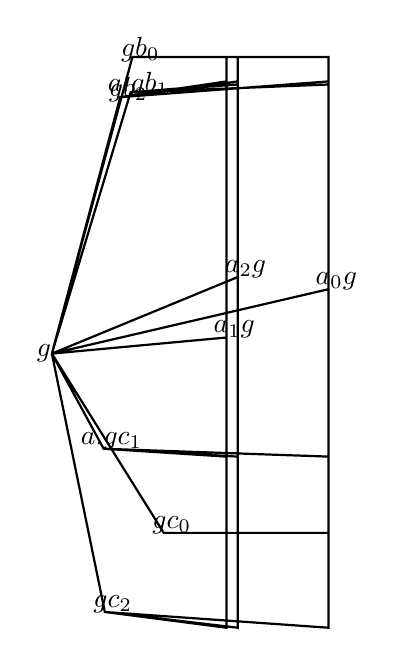
\begin{tikzpicture}
            \draw[thick](0,0)(0,0) -- (1.02287716198763,3.7656354490222768) -- (3.5128641303635577,3.7656354490222768) -- (3.5128641303635577,0.8174011386604012) -- (0,0)
(0,0) -- (0.9992014958748485,3.31737353039137) -- (3.5128641303635577,3.41737353039137) -- (3.5128641303635577,0.8174011386604012) -- (0,0)
(0,0) -- (0.868383817933343,3.256442703881467) -- (3.5128641303635577,3.4564427038814673) -- (3.5128641303635577,0.8174011386604012) -- (0,0)
(0,0) -- (1.02287716198763,3.7656354490222768) -- (2.2169741783264243,3.7656354490222768) -- (2.2169741783264243,0.2041478159768335) -- (0,0)
(0,0) -- (0.9992014958748485,3.31737353039137) -- (2.2169741783264243,3.41737353039137) -- (2.2169741783264243,0.2041478159768335) -- (0,0)
(0,0) -- (0.868383817933343,3.256442703881467) -- (2.2169741783264243,3.4564427038814673) -- (2.2169741783264243,0.2041478159768335) -- (0,0)
(0,0) -- (1.02287716198763,3.7656354490222768) -- (2.3598132908214255,3.7656354490222768) -- (2.3598132908214255,0.9717134714006355) -- (0,0)
(0,0) -- (0.9992014958748485,3.31737353039137) -- (2.3598132908214255,3.41737353039137) -- (2.3598132908214255,0.9717134714006355) -- (0,0)
(0,0) -- (0.868383817933343,3.256442703881467) -- (2.3598132908214255,3.4564427038814673) -- (2.3598132908214255,0.9717134714006355) -- (0,0)
(0,0) -- (1.4210529779529741,-2.277189261512038) -- (3.5128641303635577,-2.277189261512038) -- (3.5128641303635577,0.8174011386604012) -- (0,0)
(0,0) -- (0.6574473049549774,-1.2085179580751206) -- (3.5128641303635577,-1.3085179580751207) -- (3.5128641303635577,0.8174011386604012) -- (0,0)
(0,0) -- (0.6730537336677993,-3.28166287312954) -- (3.5128641303635577,-3.4816628731295403) -- (3.5128641303635577,0.8174011386604012) -- (0,0)
(0,0) -- (1.4210529779529741,-2.277189261512038) -- (2.2169741783264243,-2.277189261512038) -- (2.2169741783264243,0.2041478159768335) -- (0,0)
(0,0) -- (0.6574473049549774,-1.2085179580751206) -- (2.2169741783264243,-1.3085179580751207) -- (2.2169741783264243,0.2041478159768335) -- (0,0)
(0,0) -- (0.6730537336677993,-3.28166287312954) -- (2.2169741783264243,-3.4816628731295403) -- (2.2169741783264243,0.2041478159768335) -- (0,0)
(0,0) -- (1.4210529779529741,-2.277189261512038) -- (2.3598132908214255,-2.277189261512038) -- (2.3598132908214255,0.9717134714006355) -- (0,0)
(0,0) -- (0.6574473049549774,-1.2085179580751206) -- (2.3598132908214255,-1.3085179580751207) -- (2.3598132908214255,0.9717134714006355) -- (0,0)
(0,0) -- (0.6730537336677993,-3.28166287312954) -- (2.3598132908214255,-3.4816628731295403) -- (2.3598132908214255,0.9717134714006355) -- (0,0)
;
\node at (-0.1,0) {$ g $};
\node at (3.612864130363558,0.9174011386604012) {$ a_{ 0 }g $};
\node at (2.3169741783264244,0.3041478159768335) {$ a_{ 1 }g $};
\node at (2.4598132908214256,1.0717134714006356) {$ a_{ 2 }g $};
\node at (1.12287716198763,3.865635449022277) {$ gb_{ 0 } $};
\node at (1.0992014958748486,3.41737353039137) {$ a_{\cdot} gb_{ 1 } $};
\node at (0.9683838179333429,3.3564427038814673) {$ gb_{ 2 } $};
\node at (1.5210529779529742,-2.177189261512038) {$ gc_{ 0 } $};
\node at (0.7574473049549774,-1.1085179580751205) {$ a_{\cdot} gc_{ 1 } $};
\node at (0.7730537336677993,-3.18166287312954) {$ gc_{ 2 } $};

            \end{tikzpicture}
            \end{center}
            \caption{Square of the complex, with edges $(g,ag), (agb, gb) \in E_A,
            (g,gb), (agb, ag) \in E_B.$ \label{fig:square}
            }
            \end{figure}
 \begin{figure}[H]
            %\label{fig:square}
            \begin{center}
            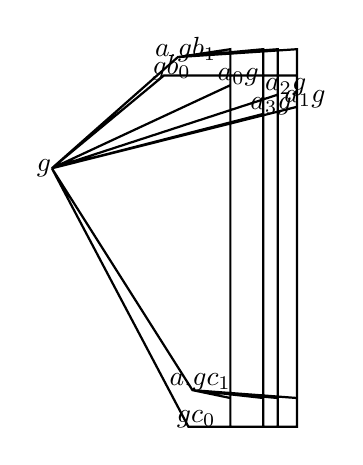
\begin{tikzpicture}
            \draw[thick](0,0)(0,0) -- (1.4214458284138272,1.177155627497069) -- (2.2669878028804726,1.177155627497069) -- (2.2669878028804726,1.0554659505060247) -- (0,0)
(0,0) -- (1.6004987782271092,1.4124264453471582) -- (2.2669878028804726,1.5124264453471583) -- (2.2669878028804726,1.0554659505060247) -- (0,0)
(0,0) -- (1.4214458284138272,1.177155627497069) -- (3.114126159828251,1.177155627497069) -- (3.114126159828251,0.7809360465448205) -- (0,0)
(0,0) -- (1.6004987782271092,1.4124264453471582) -- (3.114126159828251,1.5124264453471583) -- (3.114126159828251,0.7809360465448205) -- (0,0)
(0,0) -- (1.4214458284138272,1.177155627497069) -- (2.8697350733884743,1.177155627497069) -- (2.8697350733884743,0.9353169342269625) -- (0,0)
(0,0) -- (1.6004987782271092,1.4124264453471582) -- (2.8697350733884743,1.5124264453471583) -- (2.8697350733884743,0.9353169342269625) -- (0,0)
(0,0) -- (1.4214458284138272,1.177155627497069) -- (2.684230358001091,1.177155627497069) -- (2.684230358001091,0.6904641899615659) -- (0,0)
(0,0) -- (1.6004987782271092,1.4124264453471582) -- (2.684230358001091,1.5124264453471583) -- (2.684230358001091,0.6904641899615659) -- (0,0)
(0,0) -- (1.7335074138395734,-3.281458089103875) -- (2.2669878028804726,-3.281458089103875) -- (2.2669878028804726,1.0554659505060247) -- (0,0)
(0,0) -- (1.785365926654295,-2.8175718857238956) -- (2.2669878028804726,-2.9175718857238957) -- (2.2669878028804726,1.0554659505060247) -- (0,0)
(0,0) -- (1.7335074138395734,-3.281458089103875) -- (3.114126159828251,-3.281458089103875) -- (3.114126159828251,0.7809360465448205) -- (0,0)
(0,0) -- (1.785365926654295,-2.8175718857238956) -- (3.114126159828251,-2.9175718857238957) -- (3.114126159828251,0.7809360465448205) -- (0,0)
(0,0) -- (1.7335074138395734,-3.281458089103875) -- (2.8697350733884743,-3.281458089103875) -- (2.8697350733884743,0.9353169342269625) -- (0,0)
(0,0) -- (1.785365926654295,-2.8175718857238956) -- (2.8697350733884743,-2.9175718857238957) -- (2.8697350733884743,0.9353169342269625) -- (0,0)
(0,0) -- (1.7335074138395734,-3.281458089103875) -- (2.684230358001091,-3.281458089103875) -- (2.684230358001091,0.6904641899615659) -- (0,0)
(0,0) -- (1.785365926654295,-2.8175718857238956) -- (2.684230358001091,-2.9175718857238957) -- (2.684230358001091,0.6904641899615659) -- (0,0)
;
\node at (-0.1,0) {$ g $};
\node at (2.3669878028804727,1.1554659505060247) {$ a_{ 0 }g $};
\node at (3.214126159828251,0.8809360465448205) {$ a_{ 1 }g $};
\node at (2.9697350733884744,1.0353169342269626) {$ a_{ 2 }g $};
\node at (2.784230358001091,0.7904641899615659) {$ a_{ 3 }g $};
\node at (1.5214458284138273,1.277155627497069) {$ gb_{ 0 } $};
\node at (1.7004987782271093,1.5124264453471583) {$ a_{\cdot} gb_{ 1 } $};
\node at (1.8335074138395735,-3.181458089103875) {$ gc_{ 0 } $};
\node at (1.885365926654295,-2.7175718857238955) {$ a_{\cdot} gc_{ 1 } $};

            \end{tikzpicture}
            \end{center}
            \caption{Square of the complex, with edges $(g,ag), (agb, gb) \in E_A,
            (g,gb), (agb, ag) \in E_B.$ \label{fig:square}
            }
            \end{figure}
 \begin{figure}[H]
            %\label{fig:square}
            \begin{center}
            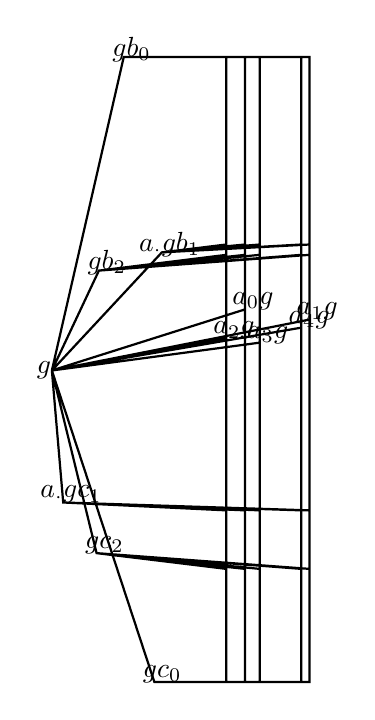
\begin{tikzpicture}
            \draw[thick](0,0)(0,0) -- (0.9128174294758034,3.9803023882107436) -- (2.45392353158174,3.9803023882107436) -- (2.45392353158174,0.7761179619415839) -- (0,0)
(0,0) -- (1.3967179429179961,1.499827435434539) -- (2.45392353158174,1.599827435434539) -- (2.45392353158174,0.7761179619415839) -- (0,0)
(0,0) -- (0.5974913836126634,1.268509718713195) -- (2.45392353158174,1.468509718713195) -- (2.45392353158174,0.7761179619415839) -- (0,0)
(0,0) -- (0.9128174294758034,3.9803023882107436) -- (3.271224645054005,3.9803023882107436) -- (3.271224645054005,0.6463752753441441) -- (0,0)
(0,0) -- (1.3967179429179961,1.499827435434539) -- (3.271224645054005,1.599827435434539) -- (3.271224645054005,0.6463752753441441) -- (0,0)
(0,0) -- (0.5974913836126634,1.268509718713195) -- (3.271224645054005,1.468509718713195) -- (3.271224645054005,0.6463752753441441) -- (0,0)
(0,0) -- (0.9128174294758034,3.9803023882107436) -- (2.2139479196807814,3.9803023882107436) -- (2.2139479196807814,0.40611877573770727) -- (0,0)
(0,0) -- (1.3967179429179961,1.499827435434539) -- (2.2139479196807814,1.599827435434539) -- (2.2139479196807814,0.40611877573770727) -- (0,0)
(0,0) -- (0.5974913836126634,1.268509718713195) -- (2.2139479196807814,1.468509718713195) -- (2.2139479196807814,0.40611877573770727) -- (0,0)
(0,0) -- (0.9128174294758034,3.9803023882107436) -- (2.6397451621916073,3.9803023882107436) -- (2.6397451621916073,0.3534541299491807) -- (0,0)
(0,0) -- (1.3967179429179961,1.499827435434539) -- (2.6397451621916073,1.599827435434539) -- (2.6397451621916073,0.3534541299491807) -- (0,0)
(0,0) -- (0.5974913836126634,1.268509718713195) -- (2.6397451621916073,1.468509718713195) -- (2.6397451621916073,0.3534541299491807) -- (0,0)
(0,0) -- (0.9128174294758034,3.9803023882107436) -- (3.1671239593021396,3.9803023882107436) -- (3.1671239593021396,0.5438183291818597) -- (0,0)
(0,0) -- (1.3967179429179961,1.499827435434539) -- (3.1671239593021396,1.599827435434539) -- (3.1671239593021396,0.5438183291818597) -- (0,0)
(0,0) -- (0.5974913836126634,1.268509718713195) -- (3.1671239593021396,1.468509718713195) -- (3.1671239593021396,0.5438183291818597) -- (0,0)
(0,0) -- (1.301170514100029,-3.95559453617341) -- (2.45392353158174,-3.95559453617341) -- (2.45392353158174,0.7761179619415839) -- (0,0)
(0,0) -- (0.14396976810945827,-1.6764045653810444) -- (2.45392353158174,-1.7764045653810445) -- (2.45392353158174,0.7761179619415839) -- (0,0)
(0,0) -- (0.5678421452854319,-2.319627186730928) -- (2.45392353158174,-2.5196271867309283) -- (2.45392353158174,0.7761179619415839) -- (0,0)
(0,0) -- (1.301170514100029,-3.95559453617341) -- (3.271224645054005,-3.95559453617341) -- (3.271224645054005,0.6463752753441441) -- (0,0)
(0,0) -- (0.14396976810945827,-1.6764045653810444) -- (3.271224645054005,-1.7764045653810445) -- (3.271224645054005,0.6463752753441441) -- (0,0)
(0,0) -- (0.5678421452854319,-2.319627186730928) -- (3.271224645054005,-2.5196271867309283) -- (3.271224645054005,0.6463752753441441) -- (0,0)
(0,0) -- (1.301170514100029,-3.95559453617341) -- (2.2139479196807814,-3.95559453617341) -- (2.2139479196807814,0.40611877573770727) -- (0,0)
(0,0) -- (0.14396976810945827,-1.6764045653810444) -- (2.2139479196807814,-1.7764045653810445) -- (2.2139479196807814,0.40611877573770727) -- (0,0)
(0,0) -- (0.5678421452854319,-2.319627186730928) -- (2.2139479196807814,-2.5196271867309283) -- (2.2139479196807814,0.40611877573770727) -- (0,0)
(0,0) -- (1.301170514100029,-3.95559453617341) -- (2.6397451621916073,-3.95559453617341) -- (2.6397451621916073,0.3534541299491807) -- (0,0)
(0,0) -- (0.14396976810945827,-1.6764045653810444) -- (2.6397451621916073,-1.7764045653810445) -- (2.6397451621916073,0.3534541299491807) -- (0,0)
(0,0) -- (0.5678421452854319,-2.319627186730928) -- (2.6397451621916073,-2.5196271867309283) -- (2.6397451621916073,0.3534541299491807) -- (0,0)
(0,0) -- (1.301170514100029,-3.95559453617341) -- (3.1671239593021396,-3.95559453617341) -- (3.1671239593021396,0.5438183291818597) -- (0,0)
(0,0) -- (0.14396976810945827,-1.6764045653810444) -- (3.1671239593021396,-1.7764045653810445) -- (3.1671239593021396,0.5438183291818597) -- (0,0)
(0,0) -- (0.5678421452854319,-2.319627186730928) -- (3.1671239593021396,-2.5196271867309283) -- (3.1671239593021396,0.5438183291818597) -- (0,0)
;
\node at (-0.1,0) {$ g $};
\node at (2.55392353158174,0.8761179619415839) {$ a_{ 0 }g $};
\node at (3.371224645054005,0.746375275344144) {$ a_{ 1 }g $};
\node at (2.3139479196807815,0.5061187757377072) {$ a_{ 2 }g $};
\node at (2.7397451621916074,0.45345412994918066) {$ a_{ 3 }g $};
\node at (3.2671239593021397,0.6438183291818597) {$ a_{ 4 }g $};
\node at (1.0128174294758034,4.080302388210743) {$ gb_{ 0 } $};
\node at (1.4967179429179962,1.599827435434539) {$ a_{\cdot} gb_{ 1 } $};
\node at (0.6974913836126634,1.3685097187131952) {$ gb_{ 2 } $};
\node at (1.401170514100029,-3.85559453617341) {$ gc_{ 0 } $};
\node at (0.24396976810945828,-1.5764045653810443) {$ a_{\cdot} gc_{ 1 } $};
\node at (0.6678421452854318,-2.219627186730928) {$ gc_{ 2 } $};

            \end{tikzpicture}
            \end{center}
            \caption{Square of the complex, with edges $(g,ag), (agb, gb) \in E_A,
            (g,gb), (agb, ag) \in E_B.$ \label{fig:square}
            }
            \end{figure}
 \begin{figure}[H]
            %\label{fig:square}
            \begin{center}
            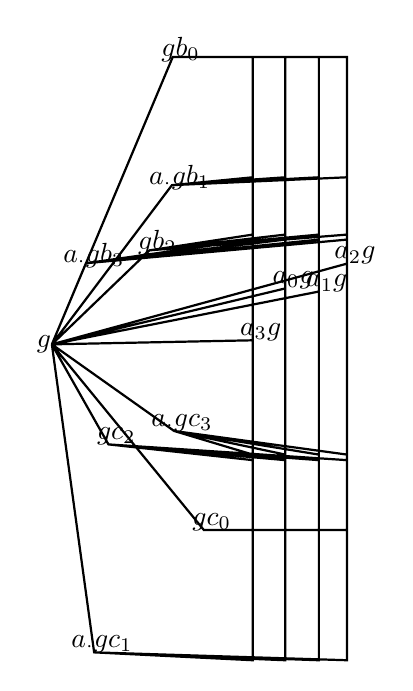
\begin{tikzpicture}
            \draw[thick](0,0)(0,0) -- (1.5349209679461768,3.64833211461554) -- (2.964968602735846,3.64833211461554) -- (2.964968602735846,0.7103627798384246) -- (0,0)
(0,0) -- (1.5244480358356187,2.0215528621236363) -- (2.964968602735846,2.1215528621236364) -- (2.964968602735846,0.7103627798384246) -- (0,0)
(0,0) -- (1.2407449652685811,1.1938472878386595) -- (2.964968602735846,1.3938472878386594) -- (2.964968602735846,0.7103627798384246) -- (0,0)
(0,0) -- (0.4324726253840361,1.0301896380962416) -- (2.964968602735846,1.3301896380962417) -- (2.964968602735846,0.7103627798384246) -- (0,0)
(0,0) -- (1.5349209679461768,3.64833211461554) -- (3.390893670392316,3.64833211461554) -- (3.390893670392316,0.670697623349611) -- (0,0)
(0,0) -- (1.5244480358356187,2.0215528621236363) -- (3.390893670392316,2.1215528621236364) -- (3.390893670392316,0.670697623349611) -- (0,0)
(0,0) -- (1.2407449652685811,1.1938472878386595) -- (3.390893670392316,1.3938472878386594) -- (3.390893670392316,0.670697623349611) -- (0,0)
(0,0) -- (0.4324726253840361,1.0301896380962416) -- (3.390893670392316,1.3301896380962417) -- (3.390893670392316,0.670697623349611) -- (0,0)
(0,0) -- (1.5349209679461768,3.64833211461554) -- (3.7486532353348725,3.64833211461554) -- (3.7486532353348725,1.0254413216319391) -- (0,0)
(0,0) -- (1.5244480358356187,2.0215528621236363) -- (3.7486532353348725,2.1215528621236364) -- (3.7486532353348725,1.0254413216319391) -- (0,0)
(0,0) -- (1.2407449652685811,1.1938472878386595) -- (3.7486532353348725,1.3938472878386594) -- (3.7486532353348725,1.0254413216319391) -- (0,0)
(0,0) -- (0.4324726253840361,1.0301896380962416) -- (3.7486532353348725,1.3301896380962417) -- (3.7486532353348725,1.0254413216319391) -- (0,0)
(0,0) -- (1.5349209679461768,3.64833211461554) -- (2.5512044061641896,3.64833211461554) -- (2.5512044061641896,0.05133191917486117) -- (0,0)
(0,0) -- (1.5244480358356187,2.0215528621236363) -- (2.5512044061641896,2.1215528621236364) -- (2.5512044061641896,0.05133191917486117) -- (0,0)
(0,0) -- (1.2407449652685811,1.1938472878386595) -- (2.5512044061641896,1.3938472878386594) -- (2.5512044061641896,0.05133191917486117) -- (0,0)
(0,0) -- (0.4324726253840361,1.0301896380962416) -- (2.5512044061641896,1.3301896380962417) -- (2.5512044061641896,0.05133191917486117) -- (0,0)
(0,0) -- (1.9307171391735578,-2.3589208906301726) -- (2.964968602735846,-2.3589208906301726) -- (2.964968602735846,0.7103627798384246) -- (0,0)
(0,0) -- (0.5367088110228997,-3.9118151205303464) -- (2.964968602735846,-4.011815120530346) -- (2.964968602735846,0.7103627798384246) -- (0,0)
(0,0) -- (0.7185207336334958,-1.270692445801425) -- (2.964968602735846,-1.470692445801425) -- (2.964968602735846,0.7103627798384246) -- (0,0)
(0,0) -- (1.5523976987313228,-1.1001818993301078) -- (2.964968602735846,-1.4001818993301078) -- (2.964968602735846,0.7103627798384246) -- (0,0)
(0,0) -- (1.9307171391735578,-2.3589208906301726) -- (3.390893670392316,-2.3589208906301726) -- (3.390893670392316,0.670697623349611) -- (0,0)
(0,0) -- (0.5367088110228997,-3.9118151205303464) -- (3.390893670392316,-4.011815120530346) -- (3.390893670392316,0.670697623349611) -- (0,0)
(0,0) -- (0.7185207336334958,-1.270692445801425) -- (3.390893670392316,-1.470692445801425) -- (3.390893670392316,0.670697623349611) -- (0,0)
(0,0) -- (1.5523976987313228,-1.1001818993301078) -- (3.390893670392316,-1.4001818993301078) -- (3.390893670392316,0.670697623349611) -- (0,0)
(0,0) -- (1.9307171391735578,-2.3589208906301726) -- (3.7486532353348725,-2.3589208906301726) -- (3.7486532353348725,1.0254413216319391) -- (0,0)
(0,0) -- (0.5367088110228997,-3.9118151205303464) -- (3.7486532353348725,-4.011815120530346) -- (3.7486532353348725,1.0254413216319391) -- (0,0)
(0,0) -- (0.7185207336334958,-1.270692445801425) -- (3.7486532353348725,-1.470692445801425) -- (3.7486532353348725,1.0254413216319391) -- (0,0)
(0,0) -- (1.5523976987313228,-1.1001818993301078) -- (3.7486532353348725,-1.4001818993301078) -- (3.7486532353348725,1.0254413216319391) -- (0,0)
(0,0) -- (1.9307171391735578,-2.3589208906301726) -- (2.5512044061641896,-2.3589208906301726) -- (2.5512044061641896,0.05133191917486117) -- (0,0)
(0,0) -- (0.5367088110228997,-3.9118151205303464) -- (2.5512044061641896,-4.011815120530346) -- (2.5512044061641896,0.05133191917486117) -- (0,0)
(0,0) -- (0.7185207336334958,-1.270692445801425) -- (2.5512044061641896,-1.470692445801425) -- (2.5512044061641896,0.05133191917486117) -- (0,0)
(0,0) -- (1.5523976987313228,-1.1001818993301078) -- (2.5512044061641896,-1.4001818993301078) -- (2.5512044061641896,0.05133191917486117) -- (0,0)
;
\node at (-0.1,0) {$ g $};
\node at (3.064968602735846,0.8103627798384245) {$ a_{ 0 }g $};
\node at (3.490893670392316,0.770697623349611) {$ a_{ 1 }g $};
\node at (3.8486532353348726,1.1254413216319392) {$ a_{ 2 }g $};
\node at (2.6512044061641897,0.15133191917486116) {$ a_{ 3 }g $};
\node at (1.634920967946177,3.74833211461554) {$ gb_{ 0 } $};
\node at (1.6244480358356188,2.1215528621236364) {$ a_{\cdot} gb_{ 1 } $};
\node at (1.3407449652685812,1.2938472878386595) {$ gb_{ 2 } $};
\node at (0.5324726253840361,1.1301896380962417) {$ a_{\cdot} gb_{ 3 } $};
\node at (2.0307171391735577,-2.2589208906301725) {$ gc_{ 0 } $};
\node at (0.6367088110228997,-3.8118151205303463) {$ a_{\cdot} gc_{ 1 } $};
\node at (0.8185207336334958,-1.170692445801425) {$ gc_{ 2 } $};
\node at (1.652397698731323,-1.0001818993301077) {$ a_{\cdot} gc_{ 3 } $};

            \end{tikzpicture}
            \end{center}
            \caption{Square of the complex, with edges $(g,ag), (agb, gb) \in E_A,
            (g,gb), (agb, ag) \in E_B.$ \label{fig:square}
            }
            \end{figure}
 
\end{multicols*}
  % \printbibliography 
\end{document}

 